\documentclass[landscape]{article}
\usepackage[margin=0.5cm]{geometry}
\usepackage{pgfplots}
\pgfplotsset{compat=1.18}

\begin{document}

\begin{figure}
\centering
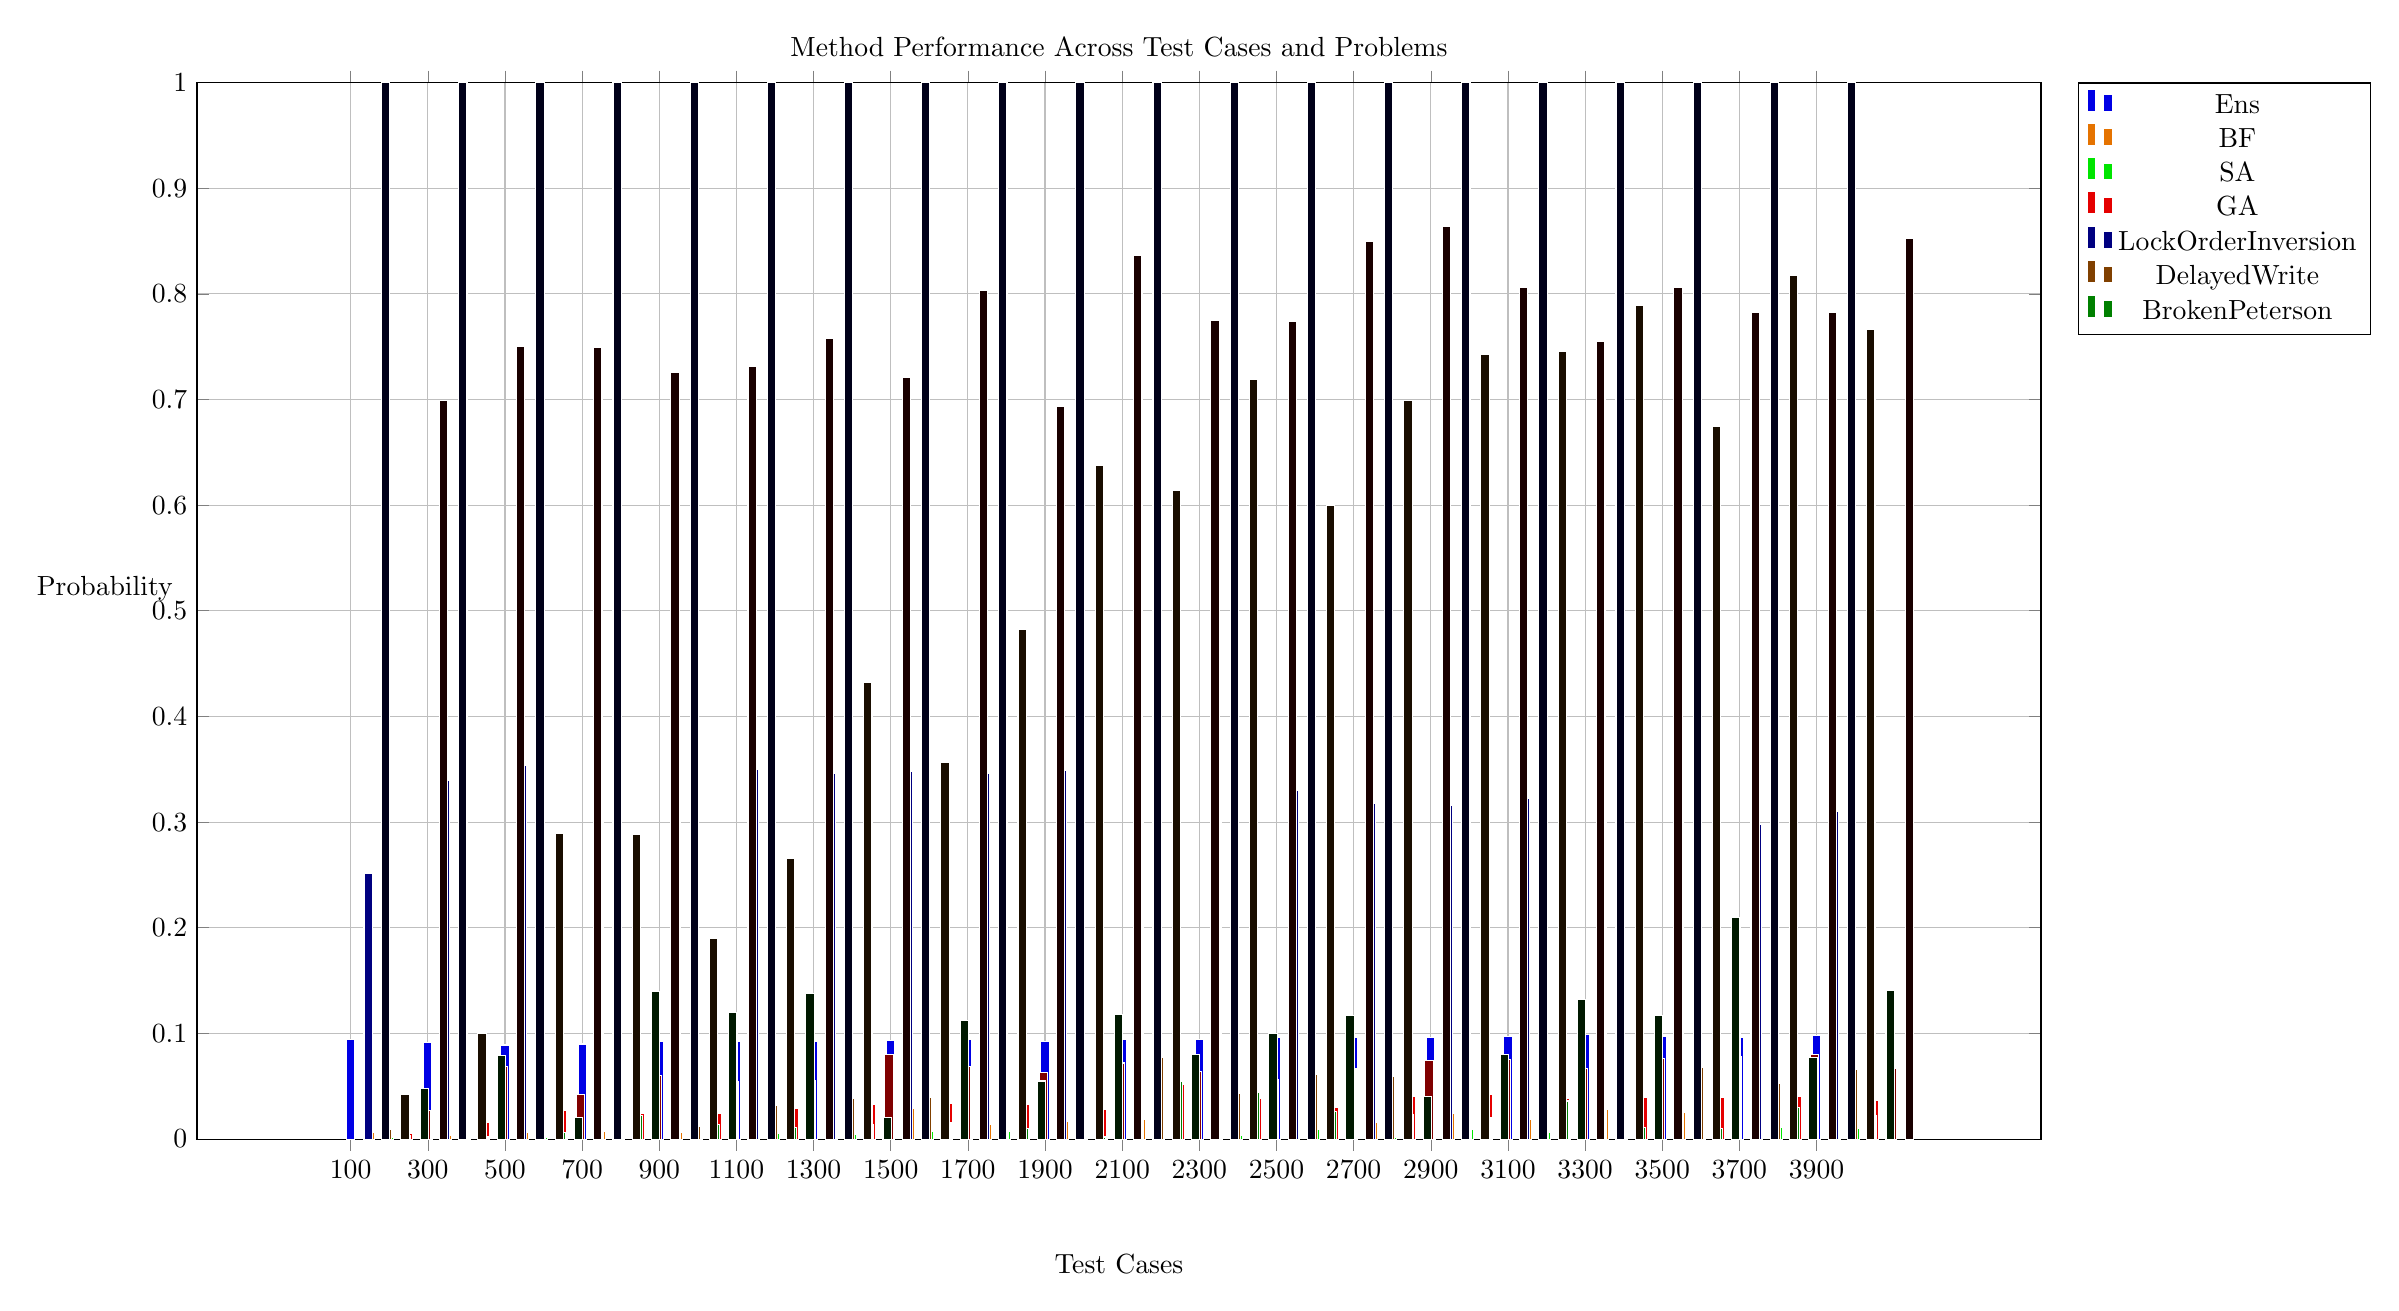
\begin{tikzpicture}
\begin{axis}[
    ybar,
    bar width=3pt,
    width=25cm,
    height=15cm,
    symbolic x coords={100-Ens-0, 100-Ens-1, 100-Ens-2, 100-BF-0, 100-BF-1, 100-BF-2, 100-SA-0, 100-SA-1, 100-SA-2, 100-GA-0, 100-GA-1, 100-GA-2, 300-Ens-0, 300-Ens-1, 300-Ens-2, 300-BF-0, 300-BF-1, 300-BF-2, 300-SA-0, 300-SA-1, 300-SA-2, 300-GA-0, 300-GA-1, 300-GA-2, 500-Ens-0, 500-Ens-1, 500-Ens-2, 500-BF-0, 500-BF-1, 500-BF-2, 500-SA-0, 500-SA-1, 500-SA-2, 500-GA-0, 500-GA-1, 500-GA-2, 700-Ens-0, 700-Ens-1, 700-Ens-2, 700-BF-0, 700-BF-1, 700-BF-2, 700-SA-0, 700-SA-1, 700-SA-2, 700-GA-0, 700-GA-1, 700-GA-2, 900-Ens-0, 900-Ens-1, 900-Ens-2, 900-BF-0, 900-BF-1, 900-BF-2, 900-SA-0, 900-SA-1, 900-SA-2, 900-GA-0, 900-GA-1, 900-GA-2, 1100-Ens-0, 1100-Ens-1, 1100-Ens-2, 1100-BF-0, 1100-BF-1, 1100-BF-2, 1100-SA-0, 1100-SA-1, 1100-SA-2, 1100-GA-0, 1100-GA-1, 1100-GA-2, 1300-Ens-0, 1300-Ens-1, 1300-Ens-2, 1300-BF-0, 1300-BF-1, 1300-BF-2, 1300-SA-0, 1300-SA-1, 1300-SA-2, 1300-GA-0, 1300-GA-1, 1300-GA-2, 1500-Ens-0, 1500-Ens-1, 1500-Ens-2, 1500-BF-0, 1500-BF-1, 1500-BF-2, 1500-SA-0, 1500-SA-1, 1500-SA-2, 1500-GA-0, 1500-GA-1, 1500-GA-2, 1700-Ens-0, 1700-Ens-1, 1700-Ens-2, 1700-BF-0, 1700-BF-1, 1700-BF-2, 1700-SA-0, 1700-SA-1, 1700-SA-2, 1700-GA-0, 1700-GA-1, 1700-GA-2, 1900-Ens-0, 1900-Ens-1, 1900-Ens-2, 1900-BF-0, 1900-BF-1, 1900-BF-2, 1900-SA-0, 1900-SA-1, 1900-SA-2, 1900-GA-0, 1900-GA-1, 1900-GA-2, 2100-Ens-0, 2100-Ens-1, 2100-Ens-2, 2100-BF-0, 2100-BF-1, 2100-BF-2, 2100-SA-0, 2100-SA-1, 2100-SA-2, 2100-GA-0, 2100-GA-1, 2100-GA-2, 2300-Ens-0, 2300-Ens-1, 2300-Ens-2, 2300-BF-0, 2300-BF-1, 2300-BF-2, 2300-SA-0, 2300-SA-1, 2300-SA-2, 2300-GA-0, 2300-GA-1, 2300-GA-2, 2500-Ens-0, 2500-Ens-1, 2500-Ens-2, 2500-BF-0, 2500-BF-1, 2500-BF-2, 2500-SA-0, 2500-SA-1, 2500-SA-2, 2500-GA-0, 2500-GA-1, 2500-GA-2, 2700-Ens-0, 2700-Ens-1, 2700-Ens-2, 2700-BF-0, 2700-BF-1, 2700-BF-2, 2700-SA-0, 2700-SA-1, 2700-SA-2, 2700-GA-0, 2700-GA-1, 2700-GA-2, 2900-Ens-0, 2900-Ens-1, 2900-Ens-2, 2900-BF-0, 2900-BF-1, 2900-BF-2, 2900-SA-0, 2900-SA-1, 2900-SA-2, 2900-GA-0, 2900-GA-1, 2900-GA-2, 3100-Ens-0, 3100-Ens-1, 3100-Ens-2, 3100-BF-0, 3100-BF-1, 3100-BF-2, 3100-SA-0, 3100-SA-1, 3100-SA-2, 3100-GA-0, 3100-GA-1, 3100-GA-2, 3300-Ens-0, 3300-Ens-1, 3300-Ens-2, 3300-BF-0, 3300-BF-1, 3300-BF-2, 3300-SA-0, 3300-SA-1, 3300-SA-2, 3300-GA-0, 3300-GA-1, 3300-GA-2, 3500-Ens-0, 3500-Ens-1, 3500-Ens-2, 3500-BF-0, 3500-BF-1, 3500-BF-2, 3500-SA-0, 3500-SA-1, 3500-SA-2, 3500-GA-0, 3500-GA-1, 3500-GA-2, 3700-Ens-0, 3700-Ens-1, 3700-Ens-2, 3700-BF-0, 3700-BF-1, 3700-BF-2, 3700-SA-0, 3700-SA-1, 3700-SA-2, 3700-GA-0, 3700-GA-1, 3700-GA-2, 3900-Ens-0, 3900-Ens-1, 3900-Ens-2, 3900-BF-0, 3900-BF-1, 3900-BF-2, 3900-SA-0, 3900-SA-1, 3900-SA-2, 3900-GA-0, 3900-GA-1, 3900-GA-2},
    xtick={100-Ens-0, 300-Ens-0, 500-Ens-0, 700-Ens-0, 900-Ens-0, 1100-Ens-0, 1300-Ens-0, 1500-Ens-0, 1700-Ens-0, 1900-Ens-0, 2100-Ens-0, 2300-Ens-0, 2500-Ens-0, 2700-Ens-0, 2900-Ens-0, 3100-Ens-0, 3300-Ens-0, 3500-Ens-0, 3700-Ens-0, 3900-Ens-0},
    xticklabels={100, 300, 500, 700, 900, 1100, 1300, 1500, 1700, 1900, 2100, 2300, 2500, 2700, 2900, 3100, 3300, 3500, 3700, 3900},
    xlabel={Test Cases},
    ylabel={Probability},
    title={Method Performance Across Test Cases and Problems},
    legend style={at={(1.02,1)}, anchor=north west},
    ymin=0,
    ymax=1,
    grid=major,
    every axis x label/.style={at={(axis description cs:0.5,-0.1)}, anchor=north},
    every axis y label/.style={at={(axis description cs:-0.05,0.5)}, anchor=south},
]


% LockOrderInversion - Ens
\addplot+[
    bar shift=0pt,
    draw=white,
    fill=black!10!blue
] coordinates {
    (100-Ens-0, 0.094) (300-Ens-0, 0.091) (500-Ens-0, 0.089) (700-Ens-0, 0.090) (900-Ens-0, 0.092) (1100-Ens-0, 0.092) (1300-Ens-0, 0.092) (1500-Ens-0, 0.093) (1700-Ens-0, 0.094) (1900-Ens-0, 0.092) (2100-Ens-0, 0.094) (2300-Ens-0, 0.094) (2500-Ens-0, 0.096) (2700-Ens-0, 0.096) (2900-Ens-0, 0.096) (3100-Ens-0, 0.097) (3300-Ens-0, 0.099) (3500-Ens-0, 0.097) (3700-Ens-0, 0.096) (3900-Ens-0, 0.098)
};

% LockOrderInversion - BF
\addplot+[
    bar shift=0pt,
    draw=white,
    fill=black!10!orange
] coordinates {
    (100-BF-0, 0.006) (300-BF-0, 0.003) (500-BF-0, 0.006) (700-BF-0, 0.007) (900-BF-0, 0.006) (1100-BF-0, 0.010) (1300-BF-0, 0.012) (1500-BF-0, 0.029) (1700-BF-0, 0.014) (1900-BF-0, 0.017) (2100-BF-0, 0.019) (2300-BF-0, 0.024) (2500-BF-0, 0.023) (2700-BF-0, 0.016) (2900-BF-0, 0.024) (3100-BF-0, 0.019) (3300-BF-0, 0.028) (3500-BF-0, 0.025) (3700-BF-0, 0.030) (3900-BF-0, 0.037)
};

% LockOrderInversion - SA
\addplot+[
    bar shift=0pt,
    draw=white,
    fill=black!10!green
] coordinates {
    (100-SA-0, 0.002) (300-SA-0, 0.001) (500-SA-0, 0.002) (700-SA-0, 0.007) (900-SA-0, 0.003) (1100-SA-0, 0.005) (1300-SA-0, 0.004) (1500-SA-0, 0.007) (1700-SA-0, 0.007) (1900-SA-0, 0.004) (2100-SA-0, 0.019) (2300-SA-0, 0.003) (2500-SA-0, 0.009) (2700-SA-0, 0.002) (2900-SA-0, 0.009) (3100-SA-0, 0.006) (3300-SA-0, 0.006) (3500-SA-0, 0.011) (3700-SA-0, 0.011) (3900-SA-0, 0.010)
};

% LockOrderInversion - GA
\addplot+[
    bar shift=0pt,
    draw=white,
    fill=black!10!red
] coordinates {
    (100-GA-0, 0.005) (300-GA-0, 0.016) (500-GA-0, 0.027) (700-GA-0, 0.024) (900-GA-0, 0.024) (1100-GA-0, 0.029) (1300-GA-0, 0.033) (1500-GA-0, 0.034) (1700-GA-0, 0.033) (1900-GA-0, 0.028) (2100-GA-0, 0.052) (2300-GA-0, 0.038) (2500-GA-0, 0.030) (2700-GA-0, 0.040) (2900-GA-0, 0.042) (3100-GA-0, 0.038) (3300-GA-0, 0.039) (3500-GA-0, 0.039) (3700-GA-0, 0.040) (3900-GA-0, 0.037)
};

% DelayedWrite - Ens
\addplot+[
    bar shift=4pt,
    draw=white,
    fill=black!50!blue
] coordinates {
    (100-Ens-1, 0.251) (300-Ens-1, 0.339) (500-Ens-1, 0.354) (700-Ens-1, 0.358) (900-Ens-1, 0.352) (1100-Ens-1, 0.350) (1300-Ens-1, 0.346) (1500-Ens-1, 0.348) (1700-Ens-1, 0.346) (1900-Ens-1, 0.349) (2100-Ens-1, 0.347) (2300-Ens-1, 0.339) (2500-Ens-1, 0.330) (2700-Ens-1, 0.318) (2900-Ens-1, 0.316) (3100-Ens-1, 0.322) (3300-Ens-1, 0.310) (3500-Ens-1, 0.323) (3700-Ens-1, 0.298) (3900-Ens-1, 0.310)
};

% DelayedWrite - BF
\addplot+[
    bar shift=4pt,
    draw=white,
    fill=black!50!orange
] coordinates {
    (100-BF-1, 0.009) (300-BF-1, 0.013) (500-BF-1, 0.013) (700-BF-1, 0.031) (900-BF-1, 0.012) (1100-BF-1, 0.032) (1300-BF-1, 0.038) (1500-BF-1, 0.039) (1700-BF-1, 0.048) (1900-BF-1, 0.053) (2100-BF-1, 0.077) (2300-BF-1, 0.043) (2500-BF-1, 0.061) (2700-BF-1, 0.059) (2900-BF-1, 0.061) (3100-BF-1, 0.056) (3300-BF-1, 0.084) (3500-BF-1, 0.068) (3700-BF-1, 0.053) (3900-BF-1, 0.066)
};

% DelayedWrite - SA
\addplot+[
    bar shift=4pt,
    draw=white,
    fill=black!50!green
] coordinates {
    (100-SA-1, 0.003) (300-SA-1, 0.002) (500-SA-1, 0.006) (700-SA-1, 0.022) (900-SA-1, 0.014) (1100-SA-1, 0.011) (1300-SA-1, 0.014) (1500-SA-1, 0.016) (1700-SA-1, 0.010) (1900-SA-1, 0.002) (2100-SA-1, 0.055) (2300-SA-1, 0.044) (2500-SA-1, 0.026) (2700-SA-1, 0.023) (2900-SA-1, 0.020) (3100-SA-1, 0.036) (3300-SA-1, 0.011) (3500-SA-1, 0.010) (3700-SA-1, 0.030) (3900-SA-1, 0.022)
};

% DelayedWrite - GA
\addplot+[
    bar shift=4pt,
    draw=white,
    fill=black!50!red
] coordinates {
    (100-GA-1, 0.027) (300-GA-1, 0.069) (500-GA-1, 0.042) (700-GA-1, 0.060) (900-GA-1, 0.054) (1100-GA-1, 0.055) (1300-GA-1, 0.080) (1500-GA-1, 0.069) (1700-GA-1, 0.063) (1900-GA-1, 0.072) (2100-GA-1, 0.064) (2300-GA-1, 0.056) (2500-GA-1, 0.067) (2700-GA-1, 0.074) (2900-GA-1, 0.075) (3100-GA-1, 0.067) (3300-GA-1, 0.076) (3500-GA-1, 0.078) (3700-GA-1, 0.080) (3900-GA-1, 0.067)
};

% BrokenPeterson - Ens
\addplot+[
    bar shift=8pt,
    draw=white,
    fill=black!90!blue
] coordinates {
    (100-Ens-2, 1.000) (300-Ens-2, 1.000) (500-Ens-2, 1.000) (700-Ens-2, 1.000) (900-Ens-2, 1.000) (1100-Ens-2, 1.000) (1300-Ens-2, 1.000) (1500-Ens-2, 1.000) (1700-Ens-2, 1.000) (1900-Ens-2, 1.000) (2100-Ens-2, 1.000) (2300-Ens-2, 1.000) (2500-Ens-2, 1.000) (2700-Ens-2, 1.000) (2900-Ens-2, 1.000) (3100-Ens-2, 1.000) (3300-Ens-2, 1.000) (3500-Ens-2, 1.000) (3700-Ens-2, 1.000) (3900-Ens-2, 1.000)
};

% BrokenPeterson - BF
\addplot+[
    bar shift=8pt,
    draw=white,
    fill=black!90!orange
] coordinates {
    (100-BF-2, 0.042) (300-BF-2, 0.100) (500-BF-2, 0.289) (700-BF-2, 0.288) (900-BF-2, 0.190) (1100-BF-2, 0.266) (1300-BF-2, 0.432) (1500-BF-2, 0.356) (1700-BF-2, 0.482) (1900-BF-2, 0.638) (2100-BF-2, 0.614) (2300-BF-2, 0.719) (2500-BF-2, 0.600) (2700-BF-2, 0.699) (2900-BF-2, 0.743) (3100-BF-2, 0.745) (3300-BF-2, 0.789) (3500-BF-2, 0.674) (3700-BF-2, 0.817) (3900-BF-2, 0.766)
};

% BrokenPeterson - SA
\addplot+[
    bar shift=8pt,
    draw=white,
    fill=black!90!green
] coordinates {
    (100-SA-2, 0.048) (300-SA-2, 0.079) (500-SA-2, 0.020) (700-SA-2, 0.140) (900-SA-2, 0.120) (1100-SA-2, 0.138) (1300-SA-2, 0.020) (1500-SA-2, 0.112) (1700-SA-2, 0.055) (1900-SA-2, 0.118) (2100-SA-2, 0.080) (2300-SA-2, 0.100) (2500-SA-2, 0.117) (2700-SA-2, 0.040) (2900-SA-2, 0.080) (3100-SA-2, 0.132) (3300-SA-2, 0.117) (3500-SA-2, 0.210) (3700-SA-2, 0.077) (3900-SA-2, 0.141)
};

% BrokenPeterson - GA
\addplot+[
    bar shift=8pt,
    draw=white,
    fill=black!90!red
] coordinates {
    (100-GA-2, 0.699) (300-GA-2, 0.750) (500-GA-2, 0.749) (700-GA-2, 0.726) (900-GA-2, 0.731) (1100-GA-2, 0.758) (1300-GA-2, 0.721) (1500-GA-2, 0.803) (1700-GA-2, 0.693) (1900-GA-2, 0.836) (2100-GA-2, 0.775) (2300-GA-2, 0.774) (2500-GA-2, 0.850) (2700-GA-2, 0.864) (2900-GA-2, 0.806) (3100-GA-2, 0.755) (3300-GA-2, 0.806) (3500-GA-2, 0.782) (3700-GA-2, 0.782) (3900-GA-2, 0.852)
};

% Legend entries
\legend{Ens, BF, SA, GA, LockOrderInversion, DelayedWrite, BrokenPeterson}

\end{axis}
\end{tikzpicture}
\caption{Method performance across test cases with different problems. Each method group shows bars for different problems, with the first input file appearing rightmost.}
\end{figure}

\end{document}